\renewcommand\labelitemii{$\m\bullet$}
\section{Étude du projet}

\subsection{Introduction}
\noindent
Dans ce premier chapitre, nous mettrons l’accent sur le cadre du projet. Par conséquent, nous commencerons par présenter l’entreprise d’accueil Axam. Par la suite, nous présenterons en détail le sujet du projet, en introduisant une vue d’ensemble du problème, une étude de l’existant et la solution proposée. Ainsi la présentation de la méthode du travail pour laquelle nous avons opté.

\subsection{Cadre du projet}
\noindent
Ce projet s’inscrit dans le cadre de projets de fin d’´etudes au sein de l’Institut Supérieur de Gestion de Sousse pour l’obtention du diplome de
licence en informatique de gestion (Business Intelligence). Il a été réalisé au sein de la start-up Axam. Ce travail est destiné à l'entreprise elle même pour l'amélioration de sa méthode de recherche des produits dans sa site-web.


\section{Présentation de l'entreprise}
\noindent
\large
Notre stage de fin d'études c'est déroulé au sein de l'entreprise << Axam >>. C'est un bureau informatique professionnel en d´eveloppement des sites web, des applications mobiles, et l'E-commerce. \\
La figure~\ref{fig:axam} représente le logo de Axam.
\begin{figure}[H]
\centering

\includegraphics[width=0.3\textwidth]{logos/axam.png}
\caption{Logo de l'entreprise d'Axam.}
\label{fig:axam}
\end{figure}

\begin{table}[H]
\centering % Center the table
\begin{tabular}{|>{\bfseries}m{5cm}|m{8cm}|}
\hline
\rowcolor{blue!20} % Coloring the header row
Nom de l’entreprise & Axam \\
\hline
Date de création & 2022 \\
\hline
Secteurs d’activité & Activités informatique / E-commerce\\
\hline
Siège & Sahline, Monastir \\
\hline
Téléphone & +216 55 220 306 \\
\hline
Adresse e-mail & contact@axam.tn \\
\hline
\end{tabular}
\caption{Fiche d’information sur Axam}
\label{tab:axam}
\end{table}
\noindent
Axam a été crée en 2022. La table~\ref{tab:axam} présente une fiche d’information sur cette entreprise.

\subsection{Secteurs d’activité}
\noindent
Axam est une boite de développement, de services informatiques, et d'E-commerce spécialisée dans:
\begin{itemize}
    \item la création et développement des applications web.
    \item la création des applications mobiles (Android et IOS).
    \item le design (web et mobile)
    \item la vente des produits sur son site e-commerce.
\end{itemize}
\section{Etude de l'éxistant}
\noindent
Cette première ètape de notre projet consitera en une analyse de l'existant, suivie d'une critique de l'existant afain de proposer notre solution comme solution aux problèmes identifiès. Nous baserons notre recherche sur des solutions existantes et opèrationnelles des marchès ecommerce existantes et cherchons à améliorer ce processus.

\subsection{Analyse de l'existant}
\noindent
Il est essentiel avant de commencer à réaliser le projet, de bien étudier et analyser les points forts et faibles des solutions existantes et envisager des améliorations. Nous nous concentrons sur le ur les processus métiers implémentés chez les autres entreprises d'ecommerce, en examinant l'efficacité de ces processus. Cette analyse nous permettra de comprendre comment améliorer les solutions existantes.

\begin{table}[H]
\centering
\begin{tabularx}{\textwidth}{|c|X|X|X|}
\hline
\rowcolor{blue!20}
\textbf{Logo} & \textbf{Description} & \textbf{Avantages} & \textbf{Inconvénients} \\
\hline
\raisebox{-\totalheight}{
\includegraphics[width=4cm,height=3.5cm]{logos/jumia.png}} & Jumia est un marketplace compléte avec un ecosystéme de paiement et livraison global & Processus de recherche généralisé et rapide pour la recherche des produits existantes. & Recherche que en Français, absence des suggestions si le produit n'existe pas. \\

\hline
\raisebox{-\totalheight}{
\includegraphics[width=4cm,height=3.5cm]{logos/tunisianet.png}} & Tunisianet est un marketplace Tunisienne des produits informatiques proposant une variété des produits et services aux clients. & Processus de recherche rapide. &  Recherche que en Français, absence des suggestions si le produit n'existe pas, et résultats non précis. \\
\hline
\raisebox{-\totalheight}{
\includegraphics[width=4cm,height=3.5cm]{logos/wamia.png}} & Wamia est un marketplace Tunisienne compléte qui offre des différents produits et services aux clients. & Processus de recherche rapide. &  Recherche que en Français, absence des suggestions si le produit n'existe pas, et résultats non précis. \\
\hline
\end{tabularx}
\caption{Comparaison des marketplaces Tunisiennes}
\label{tab:ecommerce_comparison}
\end{table}

\subsection{Critique de l'éxistant}
\noindent
Après une analyse de l'existant nous avons relevé quelques problémes tels que:

\renewcommand\labelitemi{$\bullet$}
\begin{itemize}
    \item L'absence de la recherche des produits en utilisant la langue Tunisienne (Derja) 
    \item Vitesse de recherche lente lors de la recherche d'un ou plusieurs produits.
    \item L'absence de la recherche des produits en utilisant la langue Arabe traditionnelle.
    \item Résultats de recherche non précis la plupart du temps.
\end{itemize}

\newpage
\section{Les Solutions}
\noindent
Pour résoudre les problèmes mentionnés ci-dessus, la société << Axam >> nous a proposé de développer et utiliser un modéle Sentence Transformer, en s'appuyant sur la plateforme Elasticsearch pour les clients mettre de:

\renewcommand\labelitemi{$\bullet$}
\begin{itemize}
    \item Améliorer la vitesse de recherche lors de la recherche d’un ou plusieurs produits.

    \item Améliorer la précision des résultats de recherche pour qu'ils correspondent exactement à ce que recherche le client dans les langues mentionnées ci-dessus.

    \item Pouvoir rechercher un ou plusieurs produits dans la langage Française.

    \item Pouvoir rechercher un ou plusieurs produits dans la langage Arabe en dialecte Tunisien.

    \item Pouvoir rechercher un ou plusieurs produits dans la langage Arabe Traditionnelle.
\end{itemize}
\newpage
\section{Méthodologie de développement}
\subsection{Introduction}
\noindent
Toute réalisation du projet doit être précédée d’une méthode de développement et un langage d’analyse et de conception, qui ont pour but de permettre de définir les étapes préliminaires de d´eveloppement d’un projet afin de rendre ce développement plus facile et plus flexible aux besoins et d’éviter tout retard au niveau du délai. En se basant sur ce constat, et pour une organisation adéquate de développement du projet et pour faciliter et accélérer la transformation
des besoins des utilisateurs en un systéme logiciel, nous avons opté pour l’approche SCRUM comme processus de travail et UML comme langage de modélisation.

\subsection{Méthode Adoptée: SCRUM}
\noindent
{\small\textbf{\textit{a. Définition}}}\mbox{}\\
Le principe de la méthode agile SCRUM est de concentrer l'équipe de développement sur un ensemble de fonctionnalités à réaliser de façon itérative, dans des itérations d'une durée de deux à quatre semaines, appelées des Sprints. Chaque Sprint commence par une estimation suivie d'une planification opérationnelle et se termine par une démonstration de ce qui a été achevé.

\noindent
{\small\textbf{\textit{b. Pourquoi SCRUM?}}}\mbox{}\\
Avant, le client ne voyait pas l'évolution du travail et n'était pratiquement pas impliqué pendant l'exécution de son projet. En effet, il ne pouvait pas commencer à faire des tests avant que tout soit presque fini. Par contre en Scrum, le client est de plus en plus impliqué dans le processus où il sera appelé à valider les livrables. À chaque livrable, les fonctionnalités sont en amélioration continue et le client voit régulièrement l'évolution des travaux et peut intervenir pour ajuster ses besoins.

\noindent
C'est pourquoi, Scrum vise essentiellement à optimiser la prévisibilité d'un projet et à mieux contrôler les risques.


\noindent
{\small\textbf{\textit{c. Les Artefacts SCRUM:}}}\mbox{} \\
Les artefacts Scrum sont des éléments du cadre Scrum qui matérialisent le travail à faire ou la valeur à apporter, ainsi que l'avancement du travail réalisé par l'équipe. Il existe trois artefacts tels que décrit dans le guide :

\begin{itemize}
  \item \small\textbf{Le Backlog Produit}, ou (\textit{Product backlog} en anglais) : est une liste ordonnée et en constante évolution du travail à réaliser afin d'améliorer le produit.
  
  \item \small\textbf{Le Backlog Sprint}, ou (\textit{Sprint backlog} en anglais) : Le Sprint backlog est une liste contenant les spécifications techniques pour les tâches devant être accomplis par l'équipe de développement au cours d'une période donnée (sprint).
  
  \item \small\textbf{Livraision}, ou (\textit{Delivery} en anglais) : la version du produit livrée aux parties prenantes après chaque sprint.
\end{itemize}

La Figure~\ref{fig:scrum} représente méthodologie SCRUM.

\begin{figure}[H]
\centering
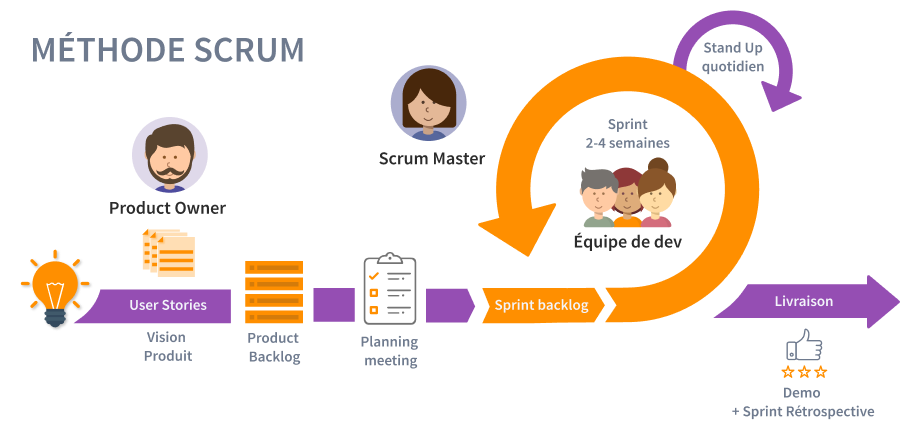
\includegraphics[width=1\textwidth]{logos/scrum.png}
\caption{Présentation du processus SCRUM}
\label{fig:scrum}
\end{figure}

\newpage
\noindent
{\small\textbf{\textit{d. Les rôles de la méthode Scrum :}}}\mbox{} \\
L'adoption de Scrum requiert la mise en place de 3 rôles spécifiques. Il s'agit du: Product owner, de l'équipe de développement et du Scrum master.

\begin{itemize}
  \item \small\textbf{Product Owner: } Le product owner (PO) représente le client ou l'utilisateur final. Son rôle est de veiller à ce que le produit soit conforme aux attentes du client que ce soit en termes de qualité ou de valeur ajoutée.
  
  \item \small\textbf{Scrum Master: } Il est le leader de l'équipe, il s'assure que le scrum est correctement appliquée et respectée et enlève les obstacles qui peuvent perturber l'avancement des travaux.
  
  \item \small\textbf{l'équipe de Développement: } L'équipe de développement est chargée de la mise en œuvre des solutions techniques et de la réalisation des développements requis.
\end{itemize}

\subsection{Le Langage UML}
\noindent
Après le choix de la méthodologie de développement, nous avons besoins d’un langage de modélisation unifiée pour la modélisation de notre projet. Pour concevoir notre système, nous avons choisi UML (Unified Modeling Language) comme un langage de modélisation qui couvre les différents vues du projet. Notre choix s’est basé sur les points forts de ce langage notamment sa standardisation et les divers diagrammes qu’il propose.

\section{Conclusion}
\noindent
Dans ce chapitre, nous avons présenté le cadre général de notre projet en déterminant la problématique et en proposant une solution. Nous avons dévoilé la méthodologie de développement et la méthode de conception qui seront utilisés dans les prochains chapitres de ce rapport et nous avons argumenté notre choix.

\newpage

% L'e-commerce, ou commerce électronique, est une composante essentielle du paysage commercial moderne, révolutionnant la manière dont les entreprises vendent des produits et comment les consommateurs les achètent. Cette forme de commerce implique la vente et l'achat de biens ou de services via Internet, offrant aux consommateurs une commodité sans précédent et aux entreprises une portée mondiale, ainsi que permettre aux entreprises de travailler et d'être ouvertes à prendre des commandes 24h/24

% \noindent
% \begin{itemize}
% \item  \textbf{L'origine de l'e-commerce: } \texttt{}{L'émergence du commerce en ligne est directement liée à l'apparition du web au début des années 1990. Le 11 août 1994, Phil Brandenberger, un habitant de Philadelphie, passe la première commande en ligne en utilisant un système de paiement sécurisé par carte bancaire. \cite{wiki:xxx}}
% \end{itemize}

